\section{Actividad 5}
En el trabajo práctico anterior se analizó espectralmente una señal compuesta por tres 
sinusoides de frecuencias 50 Hz, 120 Hz y 200 Hz, con diferentes amplitudes y fases 
(constantes). 

a) Graficar la señal total en el dominio del tiempo y en el dominio de la frecuencia 
(mediante la Transformada Rápida de Fourier, FFT). 

\bigskip
\begin{figure}[H]
\centering
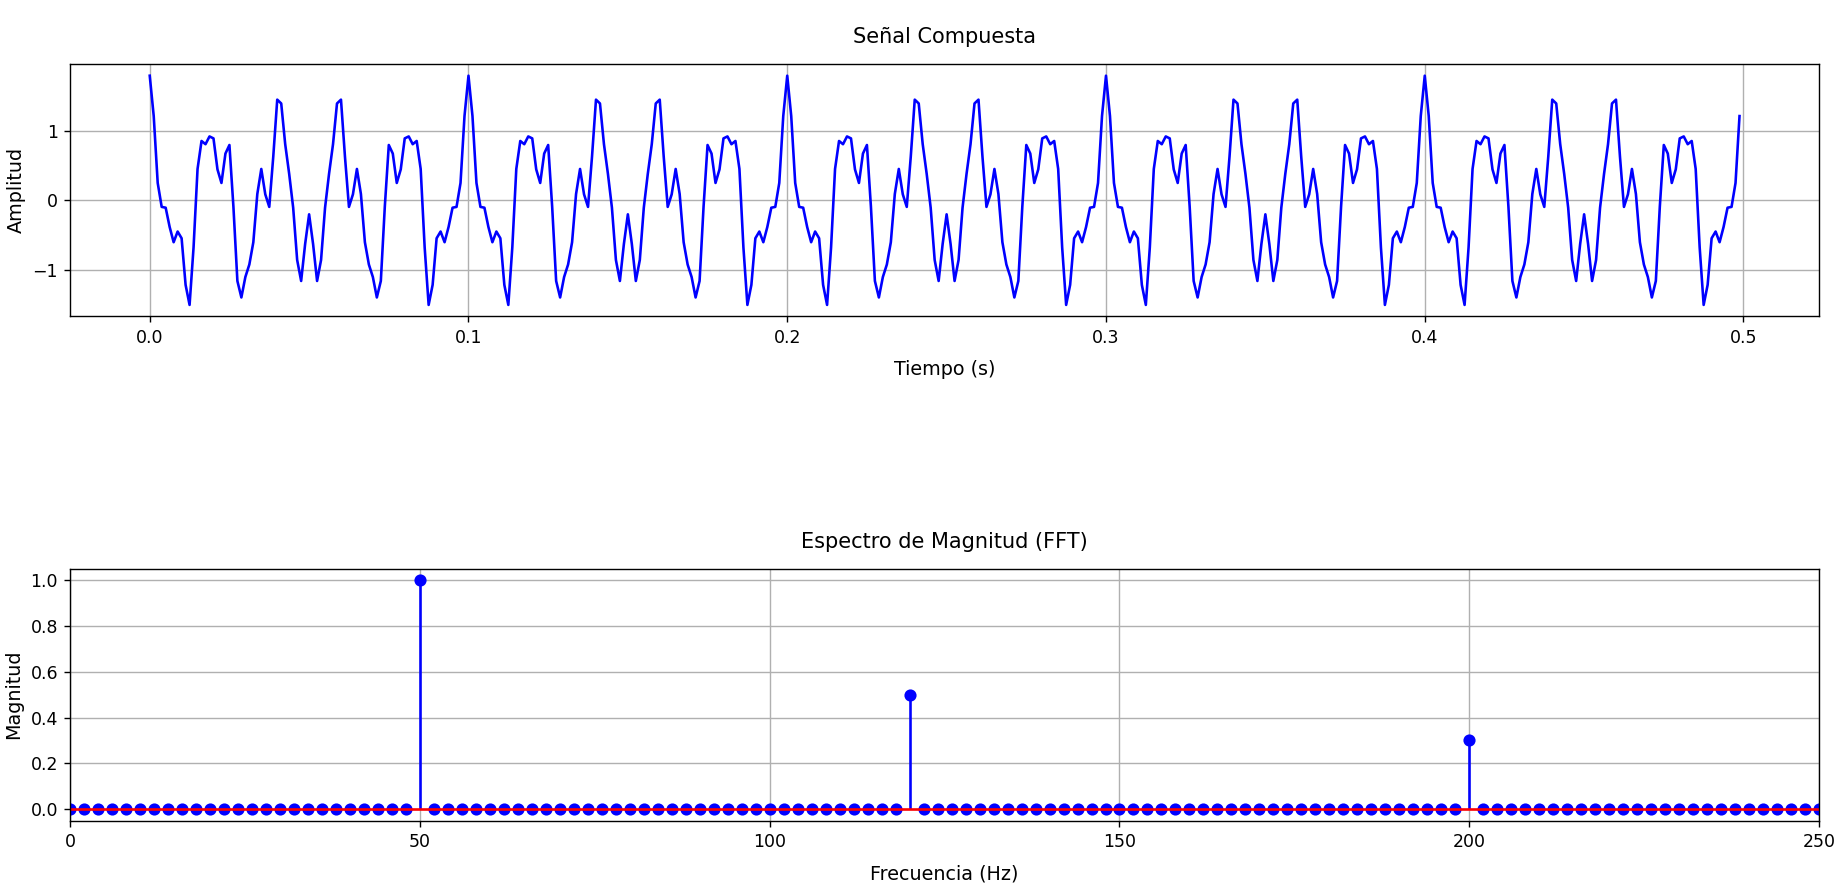
\includegraphics[width=0.8\textwidth]{parte_teorica/senalcompuesta.png}
\caption{Señal total.}
\end{figure}
\bigskip

b) Incorporar a la señal ruido blanco gaussiano en dos escenarios: 

\begin{itemize}
 \item Ruido bajo: el nivel de ruido no es suficiente para ocultar las componentes 
sinusoidales. 
 \item Ruido alto: el nivel de ruido es suficiente para enmascarar las componentes de 
la señal. 
\end{itemize}
Para cada caso, representar nuevamente la señal tanto en el tiempo como en el 
espectro de frecuencias y analizar cómo varían la visibilidad de las componentes 
espectrales. 

\bigskip
\begin{figure}[H]
\centering
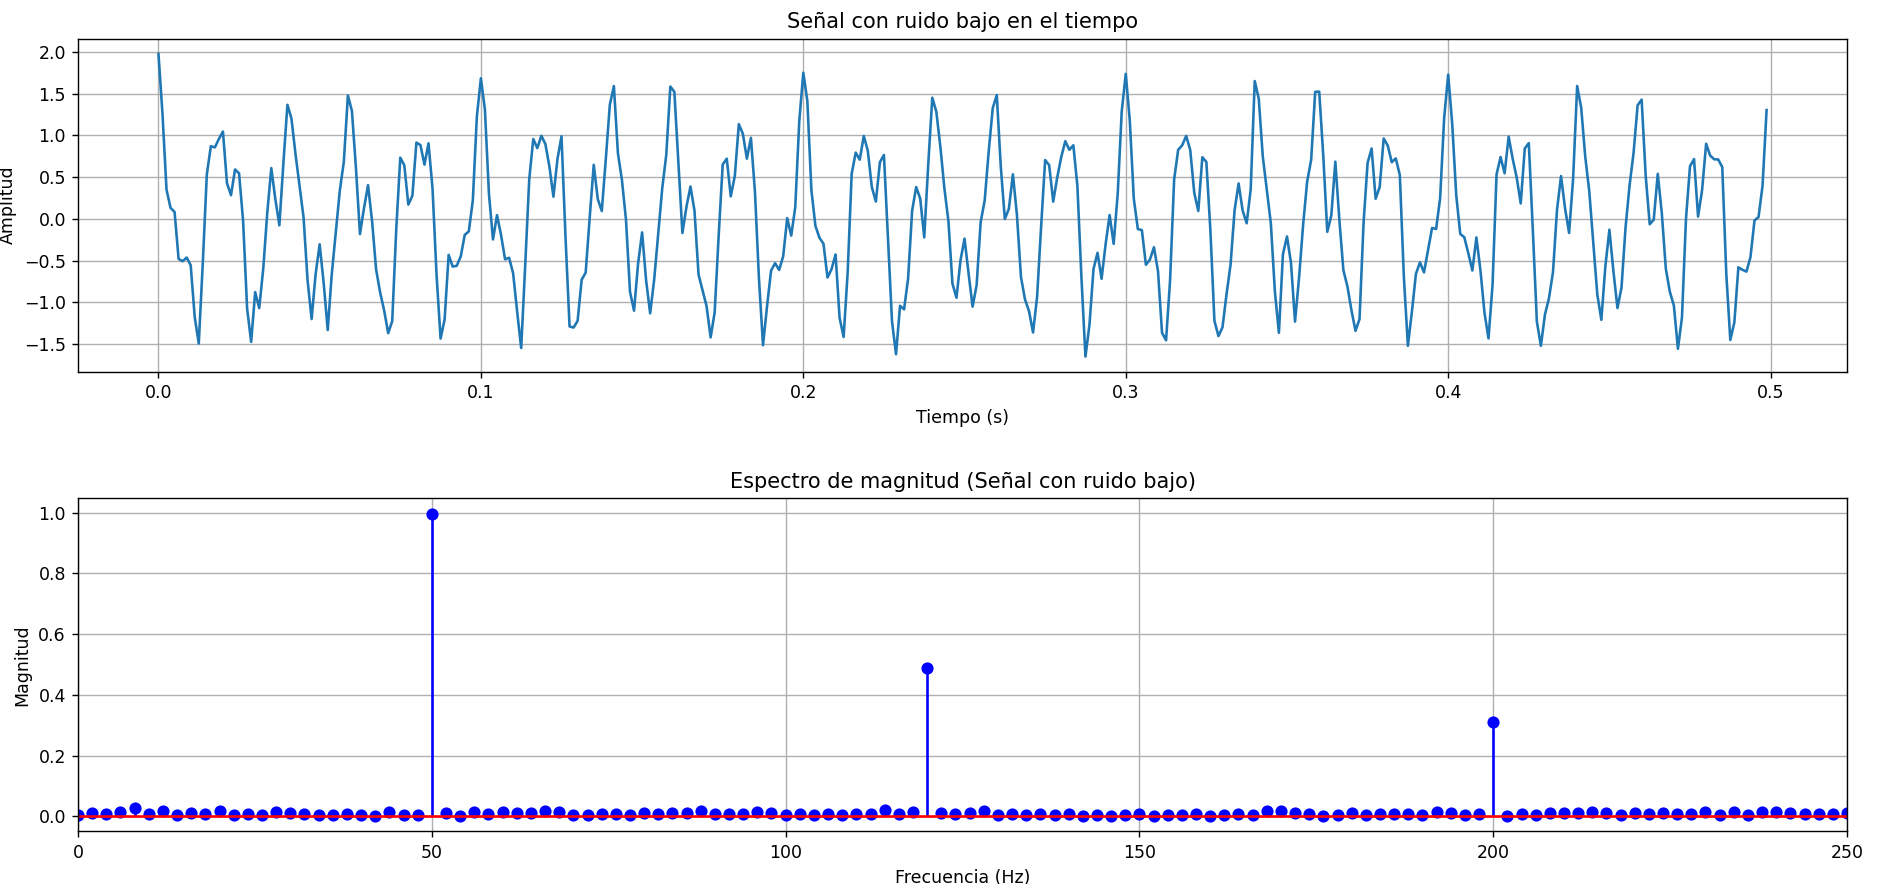
\includegraphics[width=0.8\textwidth]{parte_teorica/senalconruidobajo.png}
\caption{Señal con rudio blanco gaussiano bajo.}
\end{figure}
\bigskip

\bigskip
\begin{figure}[H]
\centering
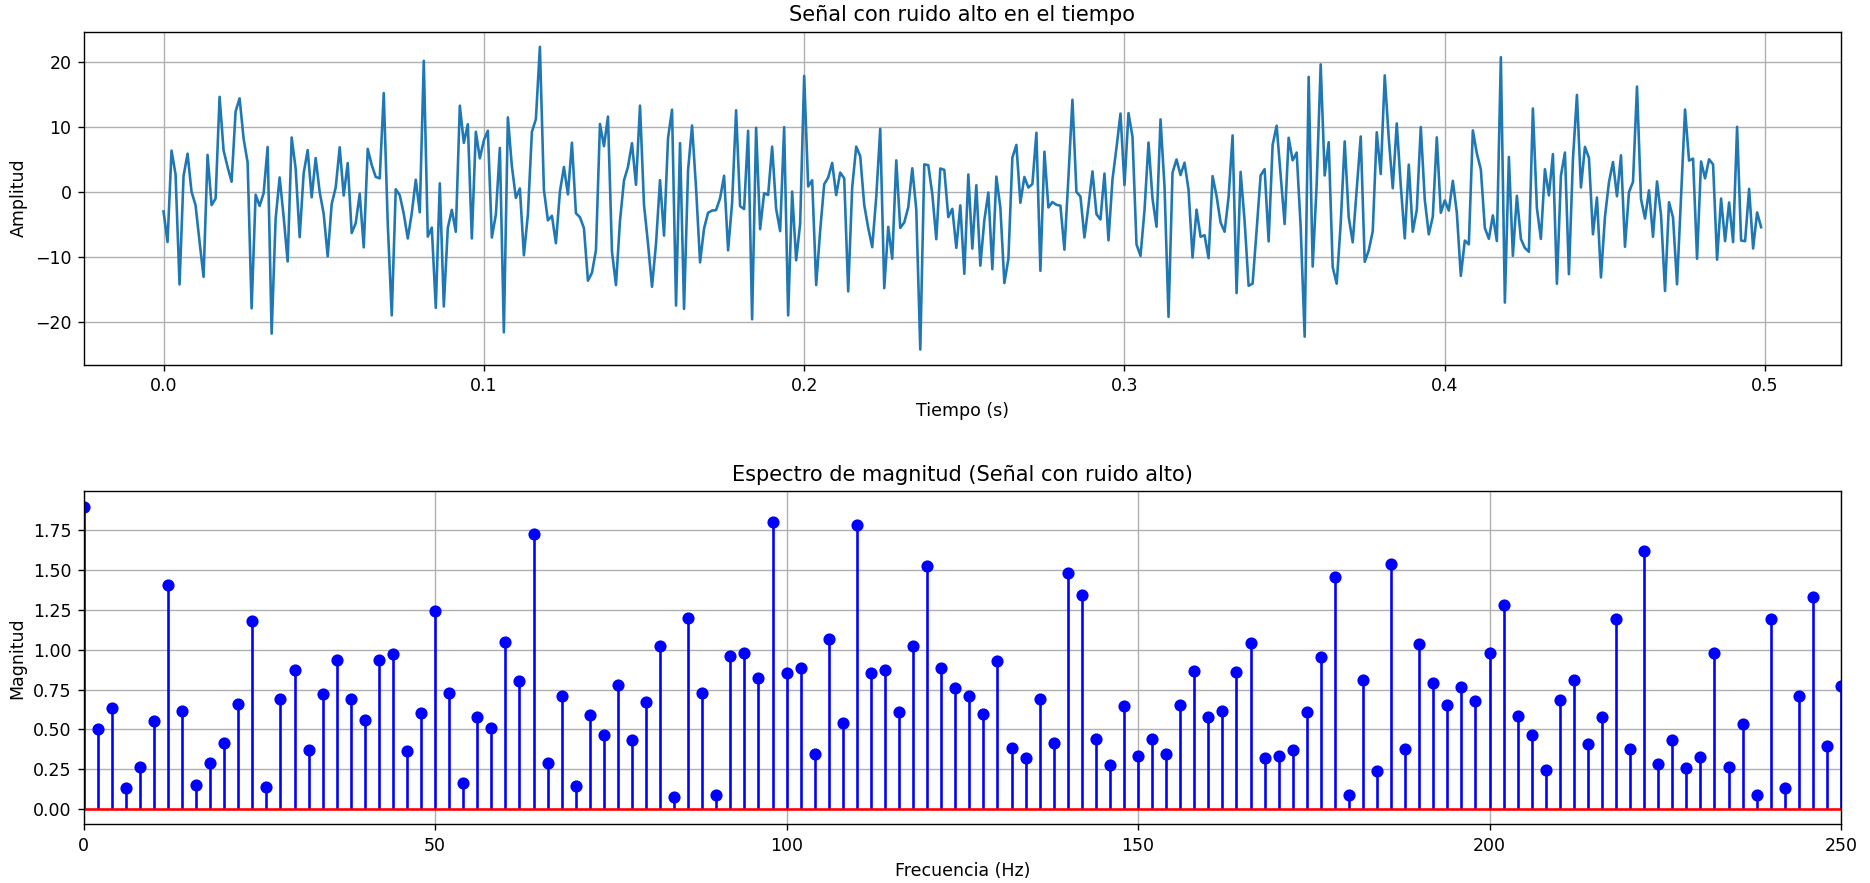
\includegraphics[width=0.8\textwidth]{parte_teorica/senalconruidoalto.png}
\caption{Señal con rudio blanco gaussiano alto.}
\end{figure}
\bigskip


Al comparar la señal original con las versiones con ruido, se observa que en el dominio del tiempo la señal total sin ruido presenta una forma suave y definida, mientras que con ruido bajo aparecen pequeñas variaciones sin perder la forma general, y con ruido alto la forma original se pierde debido a las variaciones aleatorias. En el dominio de la frecuencia, la señal total sin ruido muestra tres picos en 50 Hz, 120 Hz y 200 Hz, con las frecuencias fuera de las mencionadas en casi cero. Al añadir ruido bajo los picos siguen visibles aunque surge un nivel de ruido en todo el espectro (piso de ruido).En cambio, con ruido alto ese piso aumenta y los picos se atenúan o se confunden con el ruido. Esto quiere decir que un ruido creciente degrada la forma temporal y espectral, dificultando identificar las componentes de la señal original.

\bigskip